\documentclass{gost}

%-------------------------------------------------------------------------------
%
% ПЕРЕМЕННЫЕ
%
%-------------------------------------------------------------------------------

\newcommand{\universityFullName}{Федеральное государственное бюджетное
образовательное учреждение высшего образования Саратовский Государственный
Технический Университет имени Гагарина Ю.А.}
\newcommand{\universityShortName}{СГТУ им. Гагарина Ю.А.}
\newcommand{\department}{Прикладные информационные технологии}
\newcommand{\nirName}{Лабораторная работа по основам работы в ОС Unix}
\newcommand{\nirType}{заключительный}
\newcommand{\subject}{Программные и аппаратные технологии умного города}

%-------------------------------------------------------------------------------
%
% ДОКУМЕНТ
%
%-------------------------------------------------------------------------------

\begin{document}
	\gostTitlePage

	\section{Задание 3. Файлы и директории}
		\begin{figure}[H]
			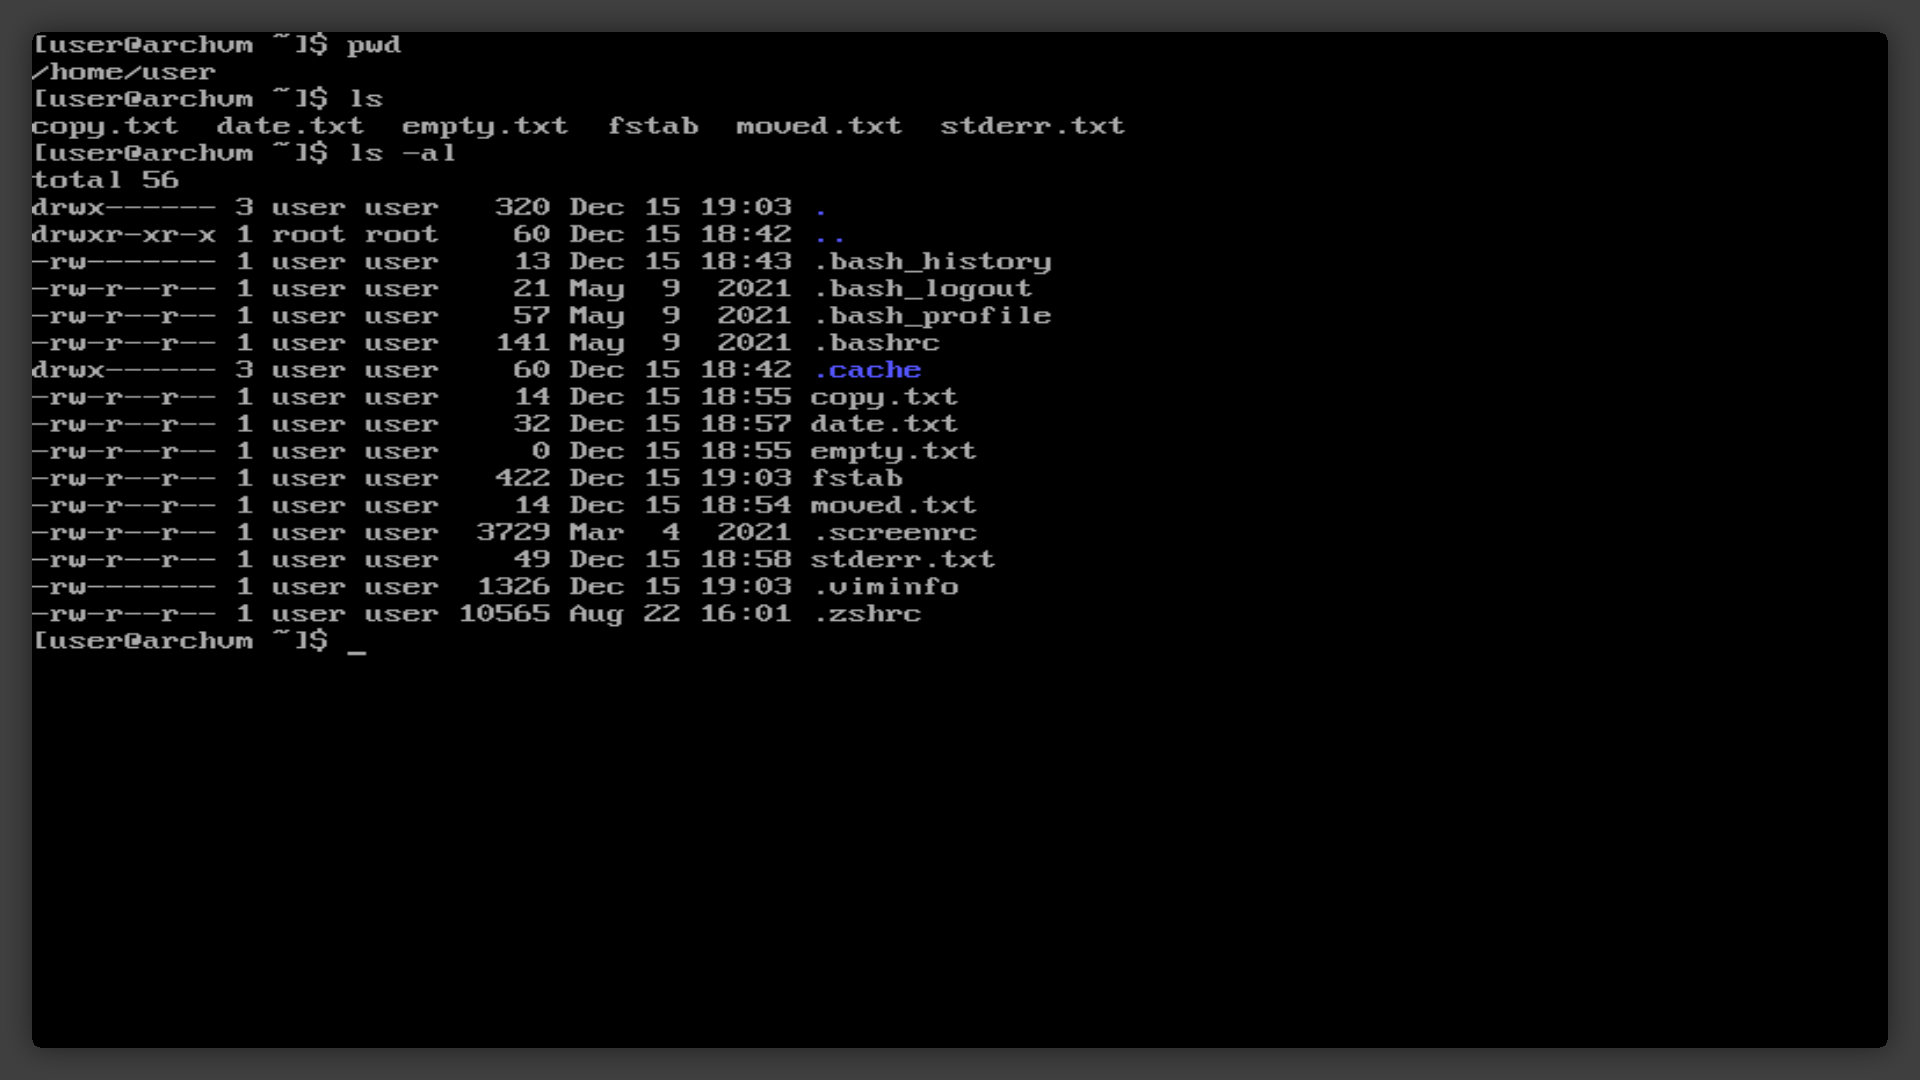
\includegraphics[width=\textwidth,clip=true]{img/1.png}
			\caption{Выводим текущий каталог, просматриваем его содержимое, а также
			содержимое с дополнительной информацией}
		\end{figure}

		\begin{figure}[H]
			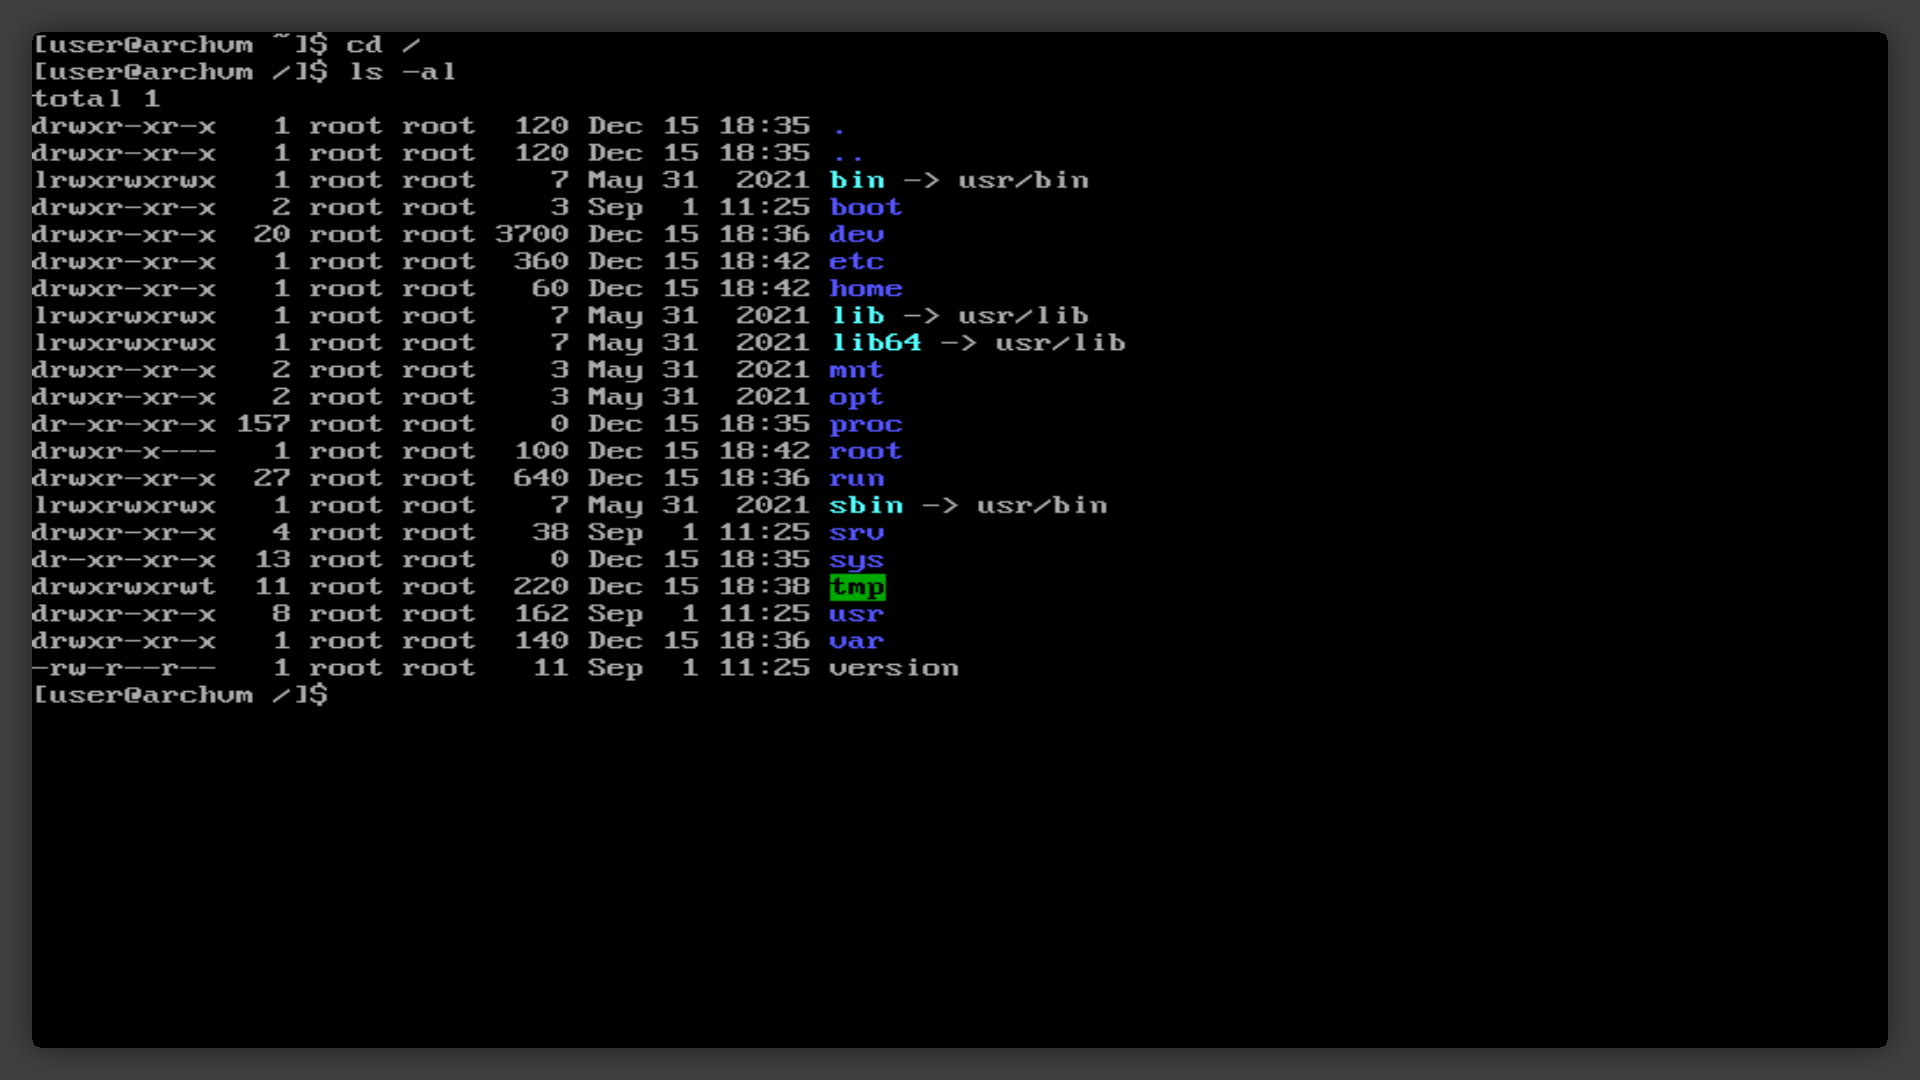
\includegraphics[width=\textwidth,clip=true]{img/2.png}
			\caption{Переходим в корневой каталог и просматриваем его содержимое}
		\end{figure}

		\begin{figure}[H]
			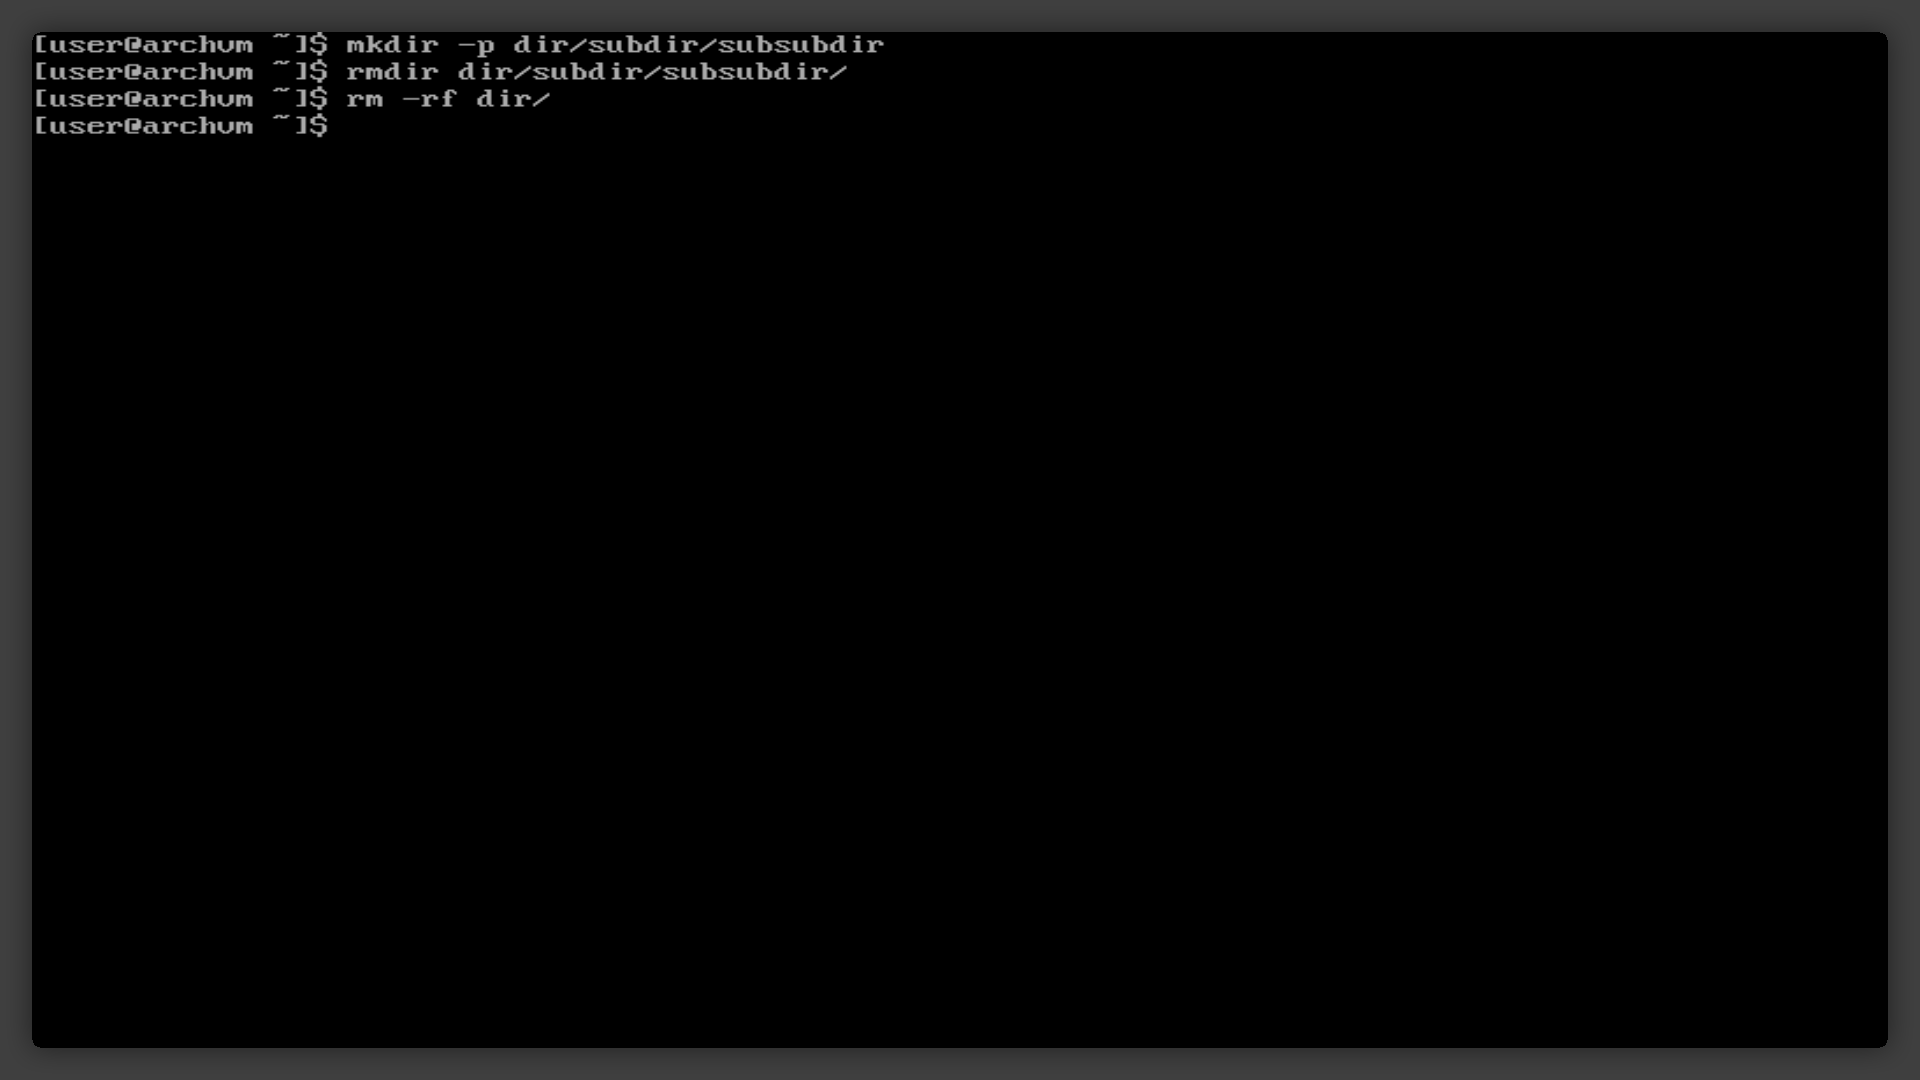
\includegraphics[width=\textwidth,clip=true]{img/3.png}
			\caption{Создаем и удаляем директории}
		\end{figure}
		
	\section{Задание 4. Операции с файлами}
		\begin{figure}[H]
			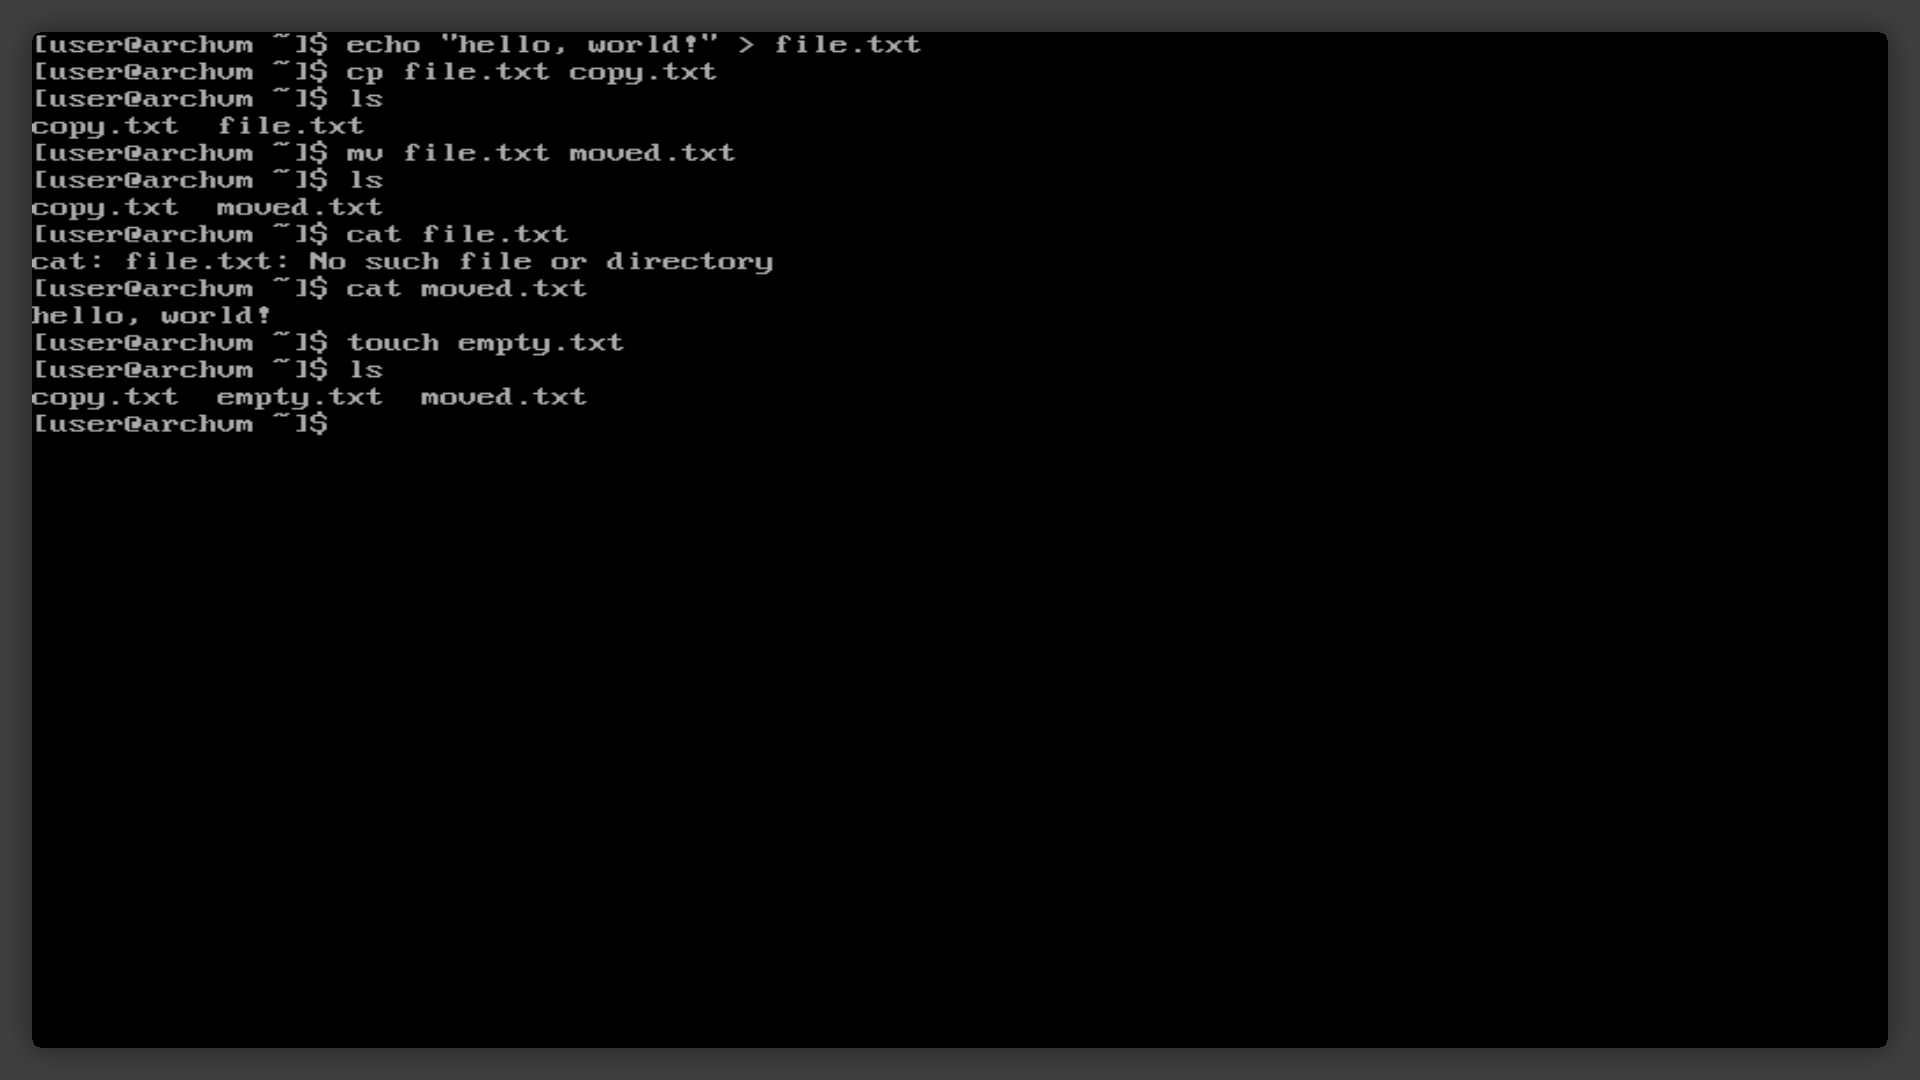
\includegraphics[width=\textwidth,clip=true]{img/4.png}
			\caption{Демонстрация простейших операций с файлами}
		\end{figure}

	\section{Задание 5. Стандартные файлы ввода-вывода}
		\begin{figure}[H]
			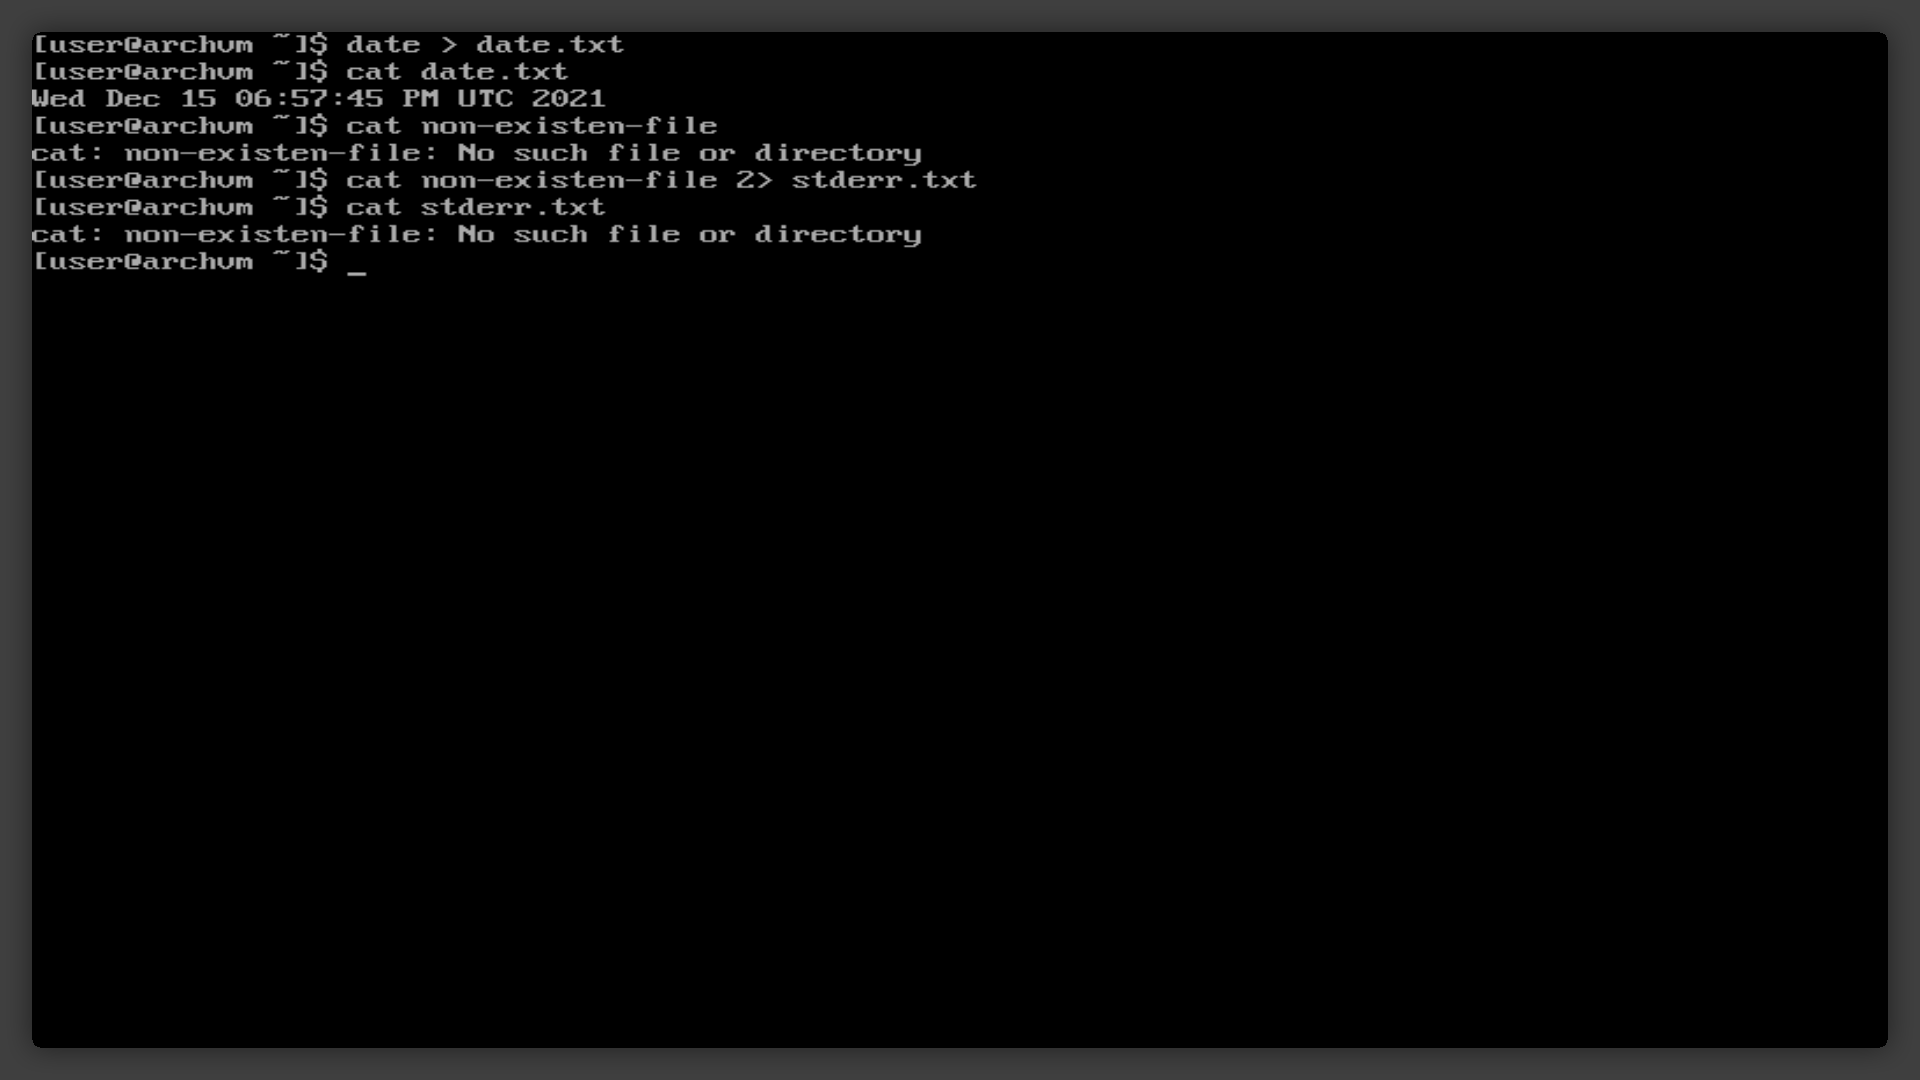
\includegraphics[width=\textwidth,clip=true]{img/5.png}
			\caption{Демонстрация работы со стандартными потоками ввода-вывода и
			перенаправлениями в командной оболочке}
		\end{figure}

	\section{Задание 6. Текстовый редактор vi}
		\begin{figure}[H]
			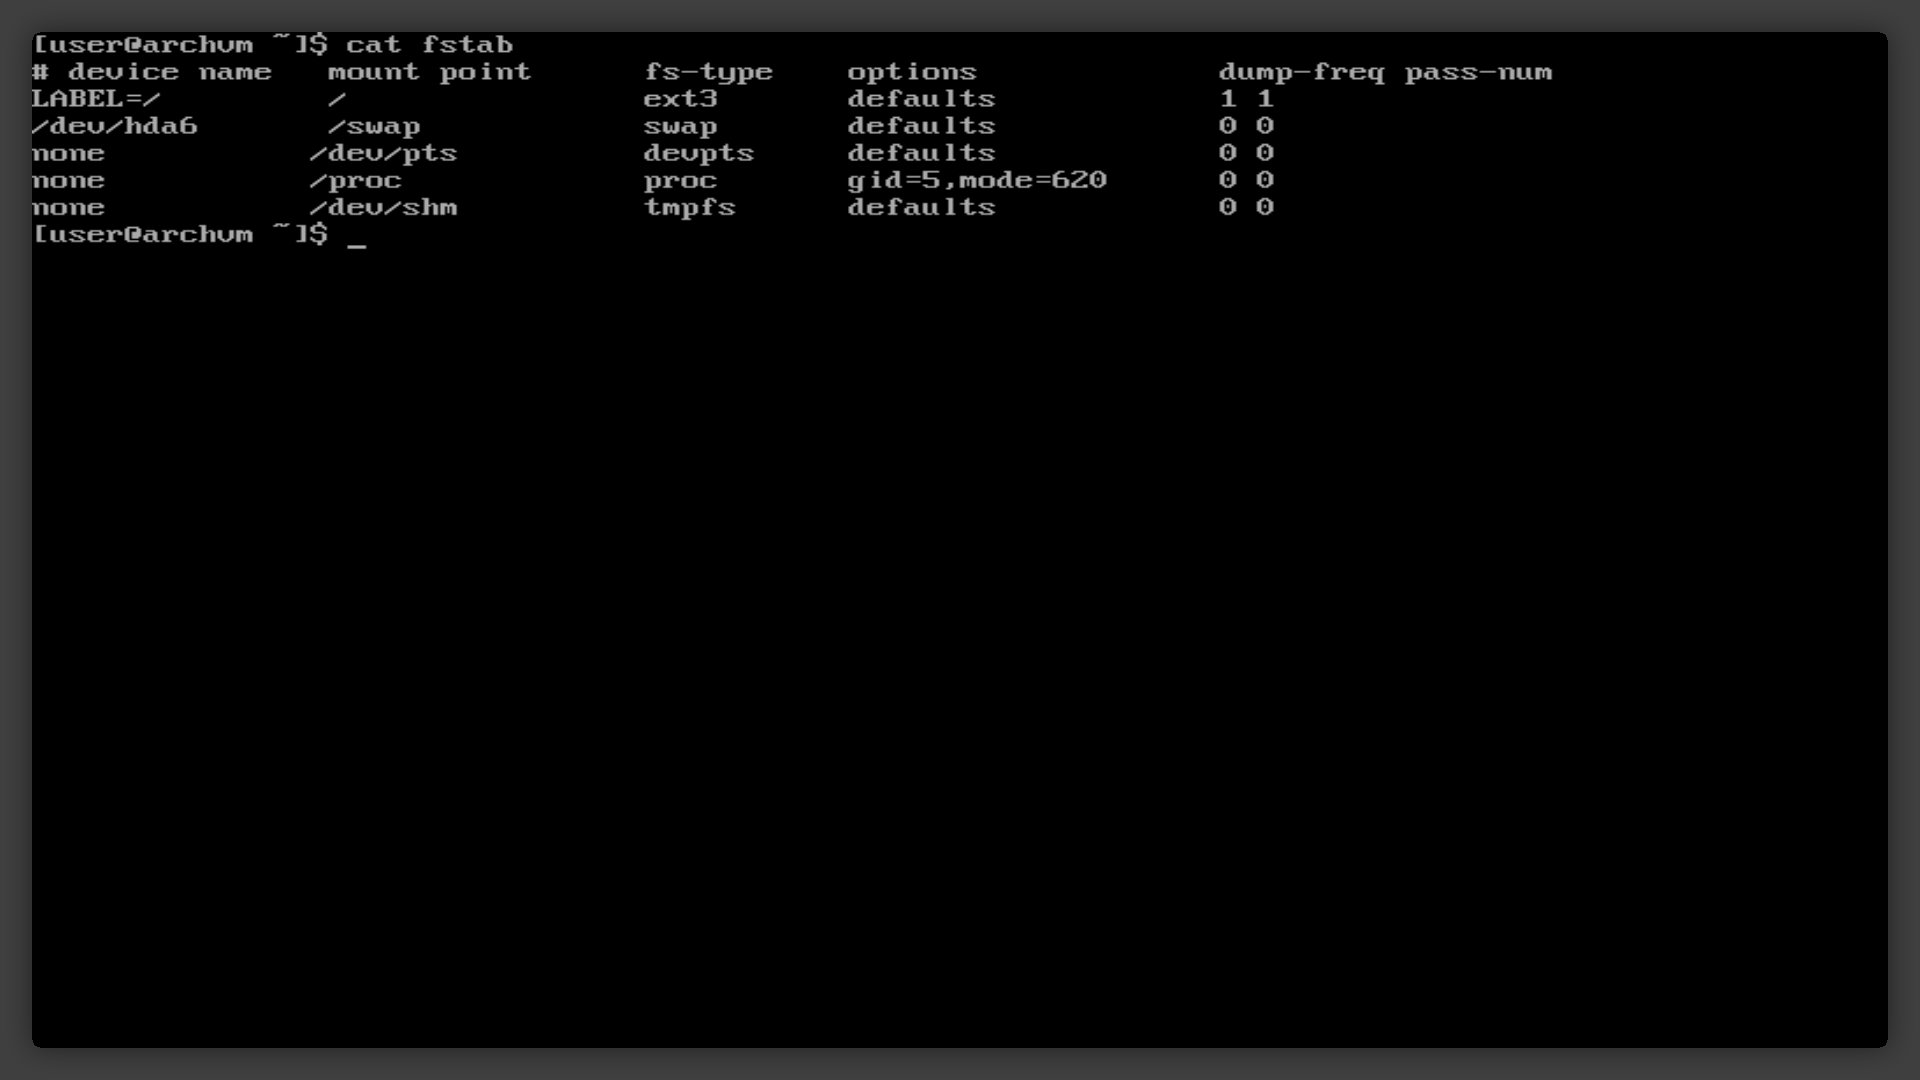
\includegraphics[width=\textwidth,clip=true]{img/6.png}
			\caption{Демонстрация работы с текстовым редактором vi}
		\end{figure}
\end{document}
